\documentclass[pdf,ps,8pt]{beamer}

\usepackage{lmodern}
\usepackage{amsmath}
\usepackage{color}
\usepackage{bbold}
\usepackage{cancel}
\usepackage{slashed}
\usepackage{graphicx}
\usepackage{verbatim}
\usepackage{textcomp}

\usetheme{Singapore}

\definecolor{palegray}{rgb}{0.82,0.822,0.82}
\newcommand{\preliminary}{
{ \rput{30}(7,-4.0){\fontsize{40}{40}\selectfont {\color{palegray}Preliminary Preliminary}} }
}

\newcommand{\textapprox}{\raisebox{0.5ex}{\texttildelow}}

\newcommand{\miniscule}{\fontsize{3pt}{4pt}\selectfont}

\def\MSbar{$\overline{\mathrm{MS}}$}
\def\gev{\,\mathrm{GeV}}
\def\mev{\,\mathrm{MeV}}
\def\fm{\,\mathrm{fm}}
\def\SU{\mathrm{SU}}
\def\su#1#2{\SU(#1)_\mathrm{#2}}
\def\rpisq{\langle r_\pi^2\rangle}
% final values
\def\rpisqsim{0.38(4)}  % pole fit for 330 MeV pion
\def\rpisqsu2sim{0.354(31)}  % su2 fit for 330 MeV pion
\def\rpisqsimlong{0.382(42)}
\def\rpisqphys{0.418(31)} % SU(2) chi extrap
\def\rpisqphyslong{0.418(31)}
\def\lsixr{-0.0093(10)} % SU(2)
\def\Lniner{0.0031(6)}  % SU(3)

\newcommand{\chpt}{\chi^{\rm PT}}
\newcommand{\tchpt}{$\chi^{\rm PT}$}
\newcommand{\tchptthree}{$\chi^{\rm PT}_3$}
\newcommand{\tchpttwo}{$\chi^{\rm PT}_2$}

\newcommand{\xiav}{\langle\,\xi\,\rangle}
\newcommand{\xisqav}{\langle\,\xi^2\,\rangle}


\newcommand{\mD}{\left(\begin{array}{cc} \DO & \Dd \\  \Ddb&\DOb \end{array} \right)}

\newcommand{\Ob}{\bar{\Omega}}

\newcommand{\DO}{D_\Omega}
\newcommand{\Dd}{D_\partial}
\newcommand{\DOi}{D_\Omega^{-1}}
\newcommand{\DOid}{D_\Omega^{-\dagger}}
\newcommand{\Pd} {\mathbb{P}_\partial}
\newcommand{\PO} {\mathbb{P}_\Omega}

\newcommand{\DOb}{D_{\bar{\Omega}}}
\newcommand{\Ddb}{D_{\bar{\partial}}}
\newcommand{\DObi}{D_{\bar{\Omega}}^{-1}}
\newcommand{\DObid}{D_{\bar{\Omega}}^{-\dagger}}
\newcommand{\Pdb}{\mathbb{P}_{\bar{\partial}}}
\newcommand{\POb} {\mathbb{P}_{\bar\Omega}}

\newcommand{\Phidb}{\mathbb{\phi}_{\bar{\partial}}}
\newcommand{\etadb}{\mathbb{\eta}_{\bar{\partial}}}

\newcommand{\hDO}{\hat D_\Omega}
\newcommand{\hDd}{\hat D_\partial}
\newcommand{\hDOi}{\hat D_\Omega^{-1}}
\newcommand{\hPd} {\hat{\mathbb{P}}_\partial}

\newcommand{\hDOb}{\hat D_{\bar{\Omega}}}
\newcommand{\hDdb}{\hat D_{\bar{\partial}}}
\newcommand{\hDObi}{\hat D_{\bar{\Omega}}^{-1}}
\newcommand{\hPdb}{\hat{\mathbb{P}}_{\bar{\partial}}}

\newcommand{\mul}[1]{\left(\begin{array}{cc}#1 & 0 \\ 0& 0\end{array}\right)}
\newcommand{\mur}[1]{\left(\begin{array}{cc}0  & #1\\ 0& 0\end{array}\right)}
\newcommand{\mll}[1]{\left(\begin{array}{cc}0  & 0 \\ #1 & 0\end{array}\right)}
\newcommand{\mlr}[1]{\left(\begin{array}{cc}0  & 0 \\ 0& #1\end{array}\right)}

\newcommand{\mDO}{\mul{ \DO}}
\newcommand{\mDd}{\mur{ \Dd}}
\newcommand{\mDOi}{\mul{\DOi}}
\newcommand{\mPd} {\mlr{\Pd}}

\newcommand{\mDOb}{\mlr{\DOb}}
\newcommand{\mDdb}{\mll{\Ddb}}
\newcommand{\mDObi}{\mlr{\DObi}}
\newcommand{\mPdb}{\mul{\Pdb}}
\newcommand{\rmod}{\mathrm{mod}}
\newcommand{\rdiv}{\mathrm{div}}

\newcommand{\link}[1]{\href{#1}{ {\color{blue} #1} }}

\beamertemplatenavigationsymbolsempty
\begin{document}


\begin{frame}[fragile]\small\frametitle{ Computational Methods (practice) -  Lecture 1    }

  \begin{center}
  
    {\color{red} Peter Boyle} (BNL, Edinburgh)
  
  \begin{itemize}
  \item Introduction \& Resources
  \item Parallel computing and data parallel programming
  \item Sparse matrices, stencils \& PDEs
  \item Example: (covariant) Laplacian
  \item Fourier tests
  \item Gauge invariance tests
  \end{itemize}

\end{center}  
\end{frame}

\begin{frame}[fragile]\small\frametitle{ Strategy  }

  \begin{itemize}
    \item Aim to give a discussion of key algorithms and topics in practical Lattice QCD simulation
    \begin{itemize}
    \item Reasonable degree of rigour, without making this a formal mathematical approach.
    \item Provide links to in depth papers and textbooks where appropriate
    \end{itemize}
    \item \emph{Will illustrate the lectures with practical examples based in Grid}
    \begin{itemize}
    \item Perhaps a unique feature of this course - let me know what works and does not work !
    \item Hope to convince you that lattice code can be small and expressive
    \end{itemize}
    \item Intersperse discussion of computing/code with discussion of algorithms/physics
    \begin{itemize}
    \item Hope this is reasonably entertaining
    \item Reflects my prejudice that computing is most efficiently learned as required to solve problems
    \end{itemize}
    \item C++ will be assumed
    \end{itemize}
\end{frame}

\begin{frame}[fragile]\small\frametitle{ Assumed programming knowledge  }

  \begin{itemize} \item C++
    \begin{itemize}
    \item operator overloading 
    \item template functions and classes - enables generic programming
    \item inheritance and object orientation
    \item Stroustroup\\
      \begin{center}\link{https://www.amazon.co.uk/C-Programming-Language-Bjarne-Stroustrup/dp/0321563840}\end{center} 
    \end{itemize}
  \item ``C'' is so much smaller than C++ it is worth learning first: Kernigan and Ritchie\\
          \begin{center}\link{https://www.amazon.co.uk/C-Programming-Language-2nd/dp/0131103628}\end{center} 
      Several keywords in C++, such as ``static'' are often misnomers, dating to ``C'' usage
  \end{itemize}
  
\end{frame}

\begin{frame}[fragile]\small\frametitle{ Why C++? }

  \begin{itemize}
  \item Low level code is possible; \\
        you can take the compiler out of the way; intrinsics, inline asm etc...
      \item High level code is possible;\\
        objects and operator overloading allow to define a mathematical type system\\
        Very high level code with natural mathematical expressions
  \item Single code base can be powerful, portable and efficient
  \item Broad based compiler support and mature standards process
  \item CUDA, HIP, SYCL are all C++ based
  \item Veldhuizen, Expression Templates: \emph{faster than fortran is possible}
  \item Templating: can write functions \& objects (matrices, vectors) of any type
    multiple precisions, Real/Complex, matrix of matrix to capture tensorial structures of QFT
  \end{itemize}

  \begin{center}
  How many ``abs'' functions do we need?
  \end{center}
  \begin{minipage}{0.5\textwidth}  
\begin{verbatim}
     #include <math.h>
     double fabs(double x);
     long double fabsl(long double x);
     float fabsf(float x);

     #include <stdlib.h>
     int   abs(int i);
     long labs(long i);
     long long llabs(long long i);
\end{verbatim}
\end{minipage}
\begin{minipage}{0.49\textwidth}  
\begin{verbatim}
     template<class t> t abs(t arg) ;
\end{verbatim}
\end{minipage}

\end{frame}


\begin{frame}[fragile]\small\frametitle{ Resources  }

  \begin{itemize} \item Computing: \end{itemize}
  \begin{center}\link{https://www.amazon.co.uk/Feynman-Lectures-Computation-Frontiers-Physics/dp/0738202967}\end{center} 
  \begin{center}\link{https://www.amazon.co.uk/Computer-Architecture-Quantitative-Approach-Kaufmann/dp/0128119055}\end{center} 
  \begin{itemize} \item Grid: \end{itemize}
  \begin{center}\link{www.github.com/paboyle/Grid}\end{center} 
  \begin{itemize} \item Grid documentation: \end{itemize}
  \begin{center}\link{https://github.com/paboyle/Grid/raw/develop/documentation/Grid.pdf}\end{center}
  \begin{itemize} \item Examples: \end{itemize}
  \begin{center}\link{https://github.com/paboyle/Grid/tree/develop/examples}\end{center}
  \begin{itemize} \item More formal courses\end{itemize}
  \begin{itemize}\item Tony Kennedy Nara lectures\end{itemize}
  \begin{center}\link{https://arxiv.org/abs/hep-lat/0607038}\end{center}
  \begin{itemize}
  \item Iterative Methods for Sparse Linear Systems, Saad
  \begin{center}
  \href{https://www-users.cse.umn.edu/~saad/IterMethBook_2ndEd.pdf}{https://www-users.cse.umn.edu/\textapprox saad/IterMethBook\_2ndEd.pdf}
  \end{center}
    \end{itemize}
\end{frame}

\begin{frame}[fragile]\small\frametitle{ Parallel computing and data parallel programming}
  \begin{itemize}
  \item Comprised of many computing nodes with programmed \emph{message passing} between nodes
  \item Distributed memory MIMD architecture / loosely coupled multiprocessors
  \begin{itemize}
  \item Complicated, cooperative access scheme for the data access (send/receive calls)
  \item Standardised by: Message Passing Interface (MPI).
  \item Predecessors: PVM.
  \item Alternatives: UPC, PGAS \verb1 Array[node][offset] 1
  \end{itemize}
  \item Nodes themselves contain many layers of parallelism
  \begin{itemize}
  \item Multiple cores of same type and multiple sockets 
  \item Accelerators (``vector'' cores of different type in a plug-in device)
  \item Two or more distinct memory spaces and instruction sets in same programme
  \item Multiple vendor supported APIs: CUDA/Nvidia; HIP/AMD; OneAPI/Intel
  \item Portability barrier(!)  
  \end{itemize}
  \end{itemize}
\end{frame}

\begin{frame}[fragile]\small\frametitle{ Parallel computing and data parallel programming}
  \begin{itemize}
  \item {\bf Modern supercomputers are increasingly difficult to programme}
  \begin{itemize}
  \item This is not the way things used to be, nor in my view the way things should be
  \end{itemize}
  \item Basic physics dictates that large computers are massively parallel and only locally well interconnected
  \begin{itemize}
  \item Wires can be long and slow or short and fast (aspect ratio dictates RC delay)
  \item Chips must be locally divided into cores
  \item ``Memory'' can be small and fast OR big and slow $\Rightarrow$ caches
  \item 3D ``Memory'', HBM and hierarchical memory
  \item Interconnect is over a few large high speed wires (or optical transceivers).
  \end{itemize}
  \end{itemize}
  \begin{center}
    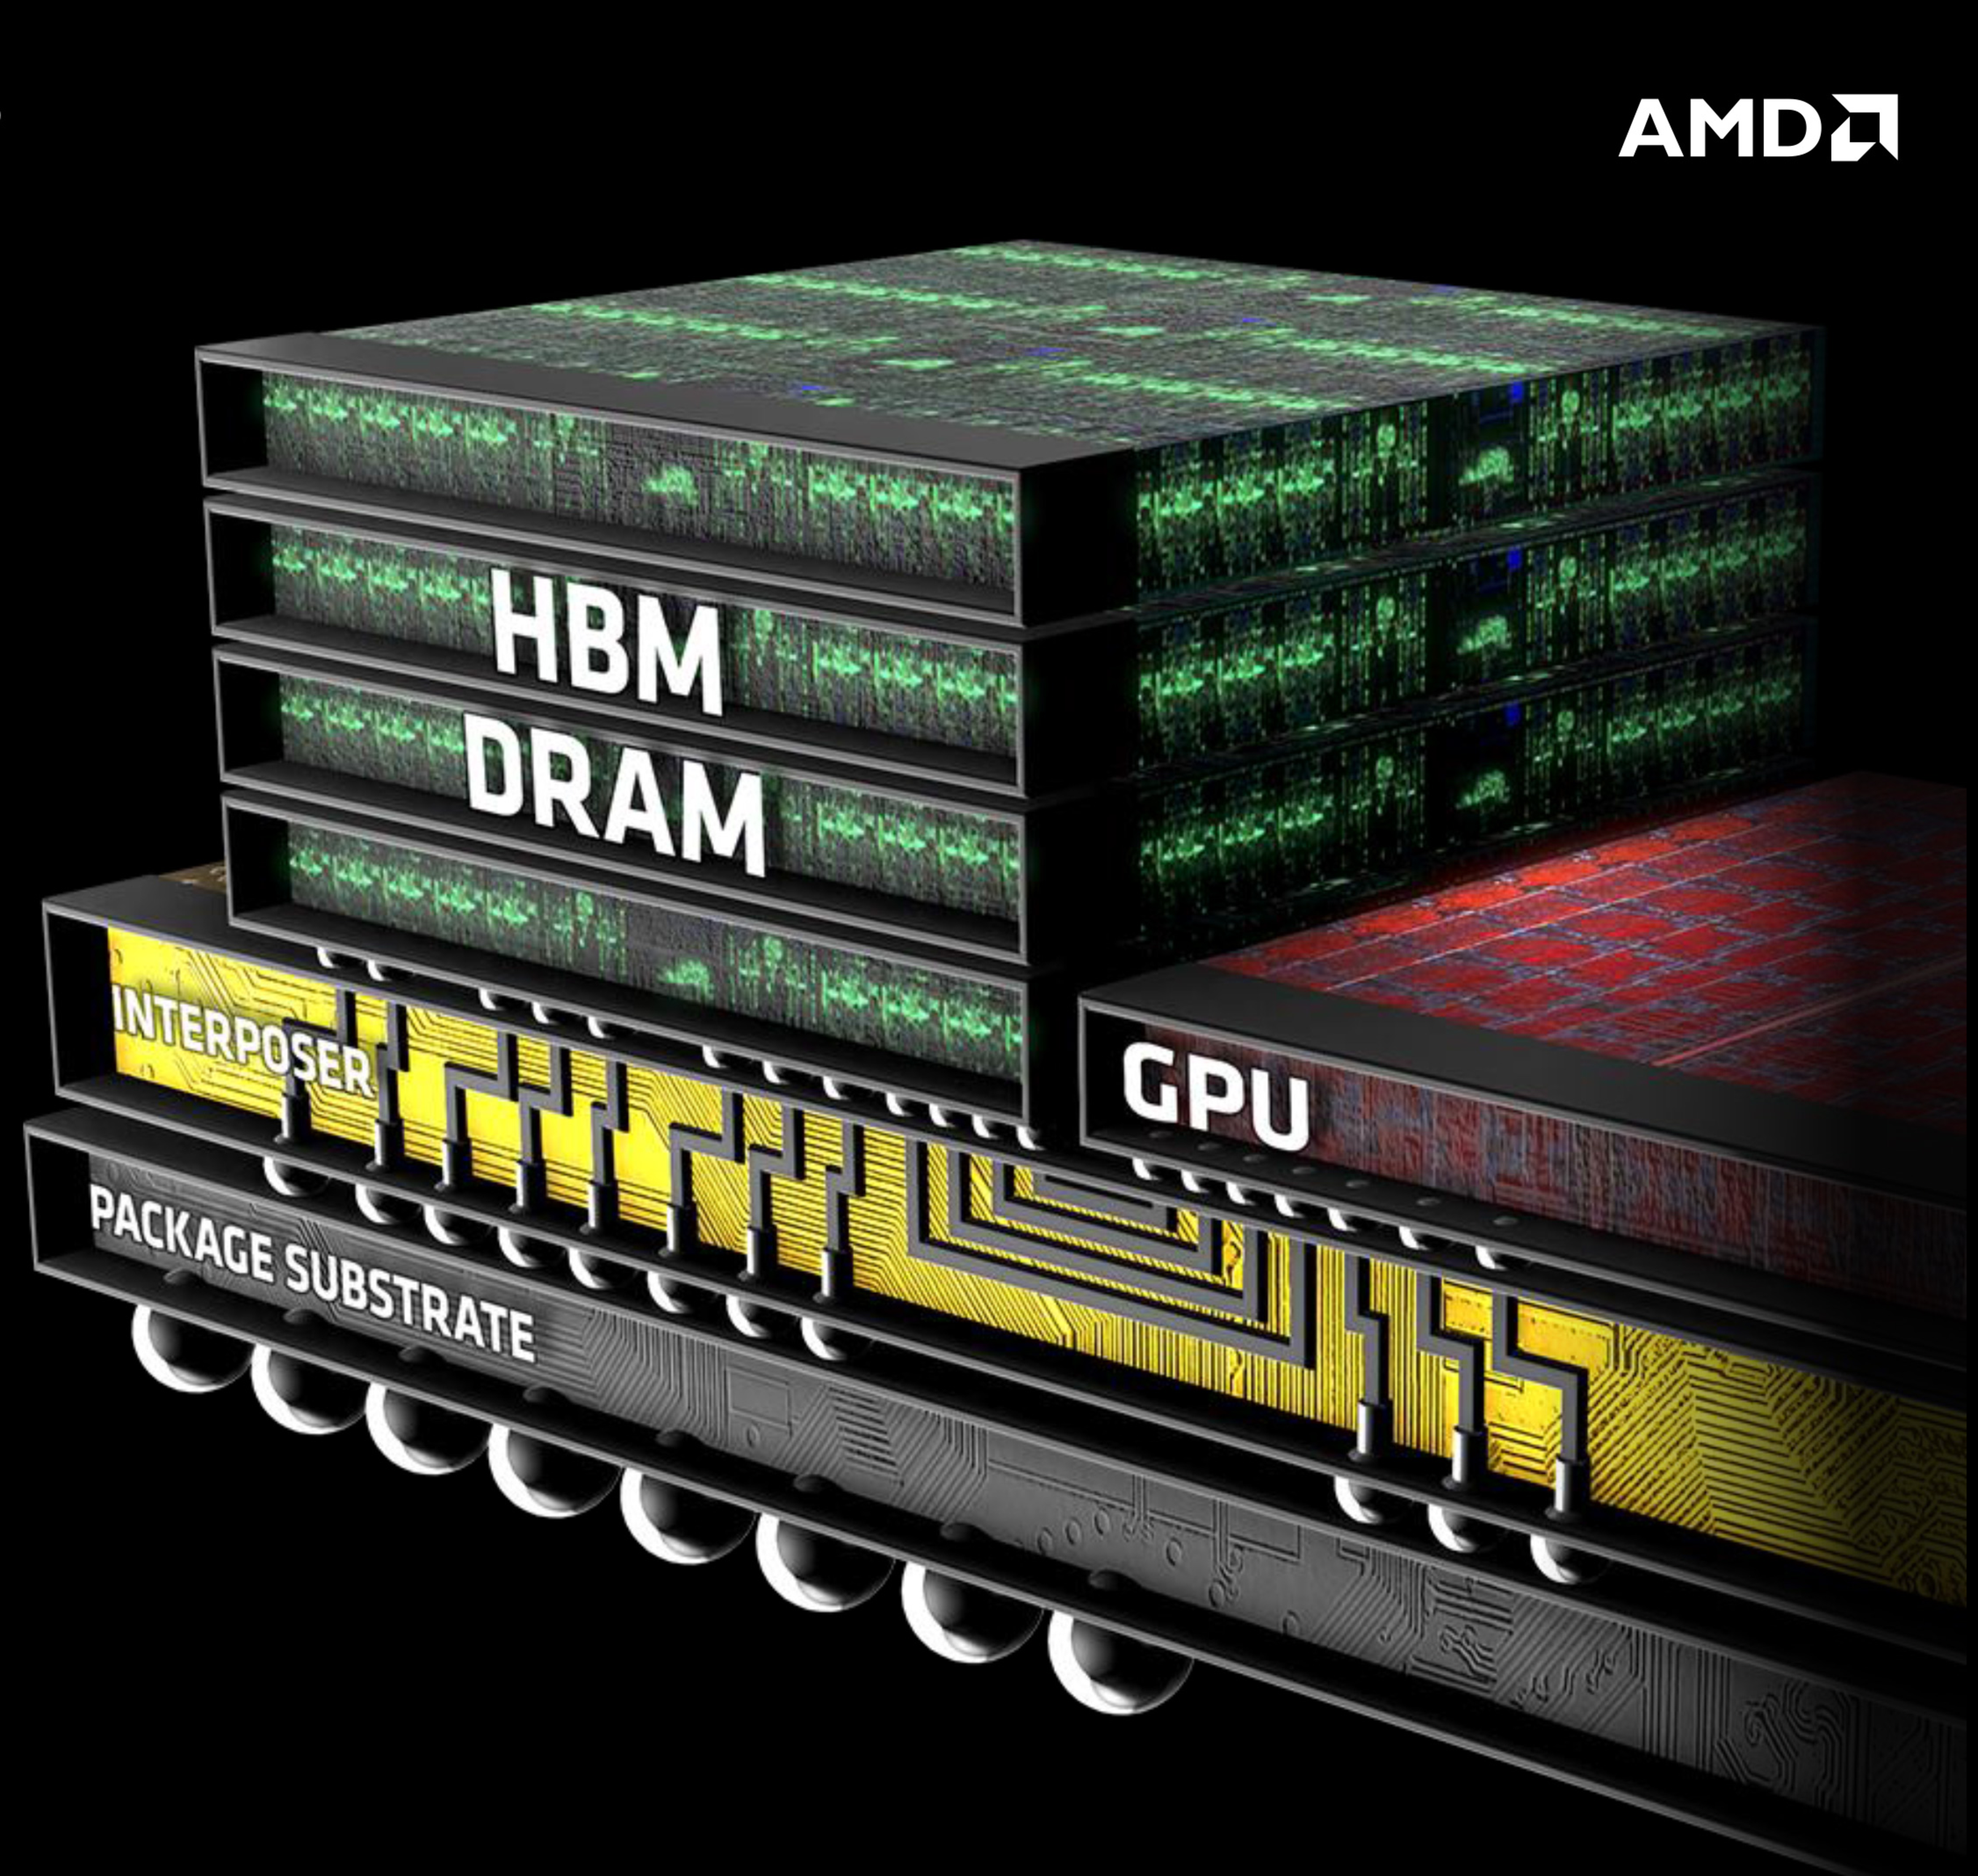
\includegraphics[width=0.4\textwidth]{HBM.pdf}
    \includegraphics[width=0.49\textwidth]{TursaNode.pdf}
    \end{center}
\end{frame}

\begin{frame}[fragile]\small\frametitle{ Parallel computing and data parallel programming}

\begin{columns}
\begin{column}{0.5\textwidth}
  \includegraphics[width=.5\textwidth]{noparitygeom1.pdf}
\end{column}
\begin{column}{0.5\textwidth}
  \includegraphics[width=\textwidth]{Aurora.jpeg}
\end{column}
\end{columns}
\begin{center}
  \includegraphics[width=0.75\textwidth]{TursaSystem.pdf}
\end{center}
\end{frame}

\begin{frame}[fragile]\small\frametitle{ Forthcoming Exascale computers}
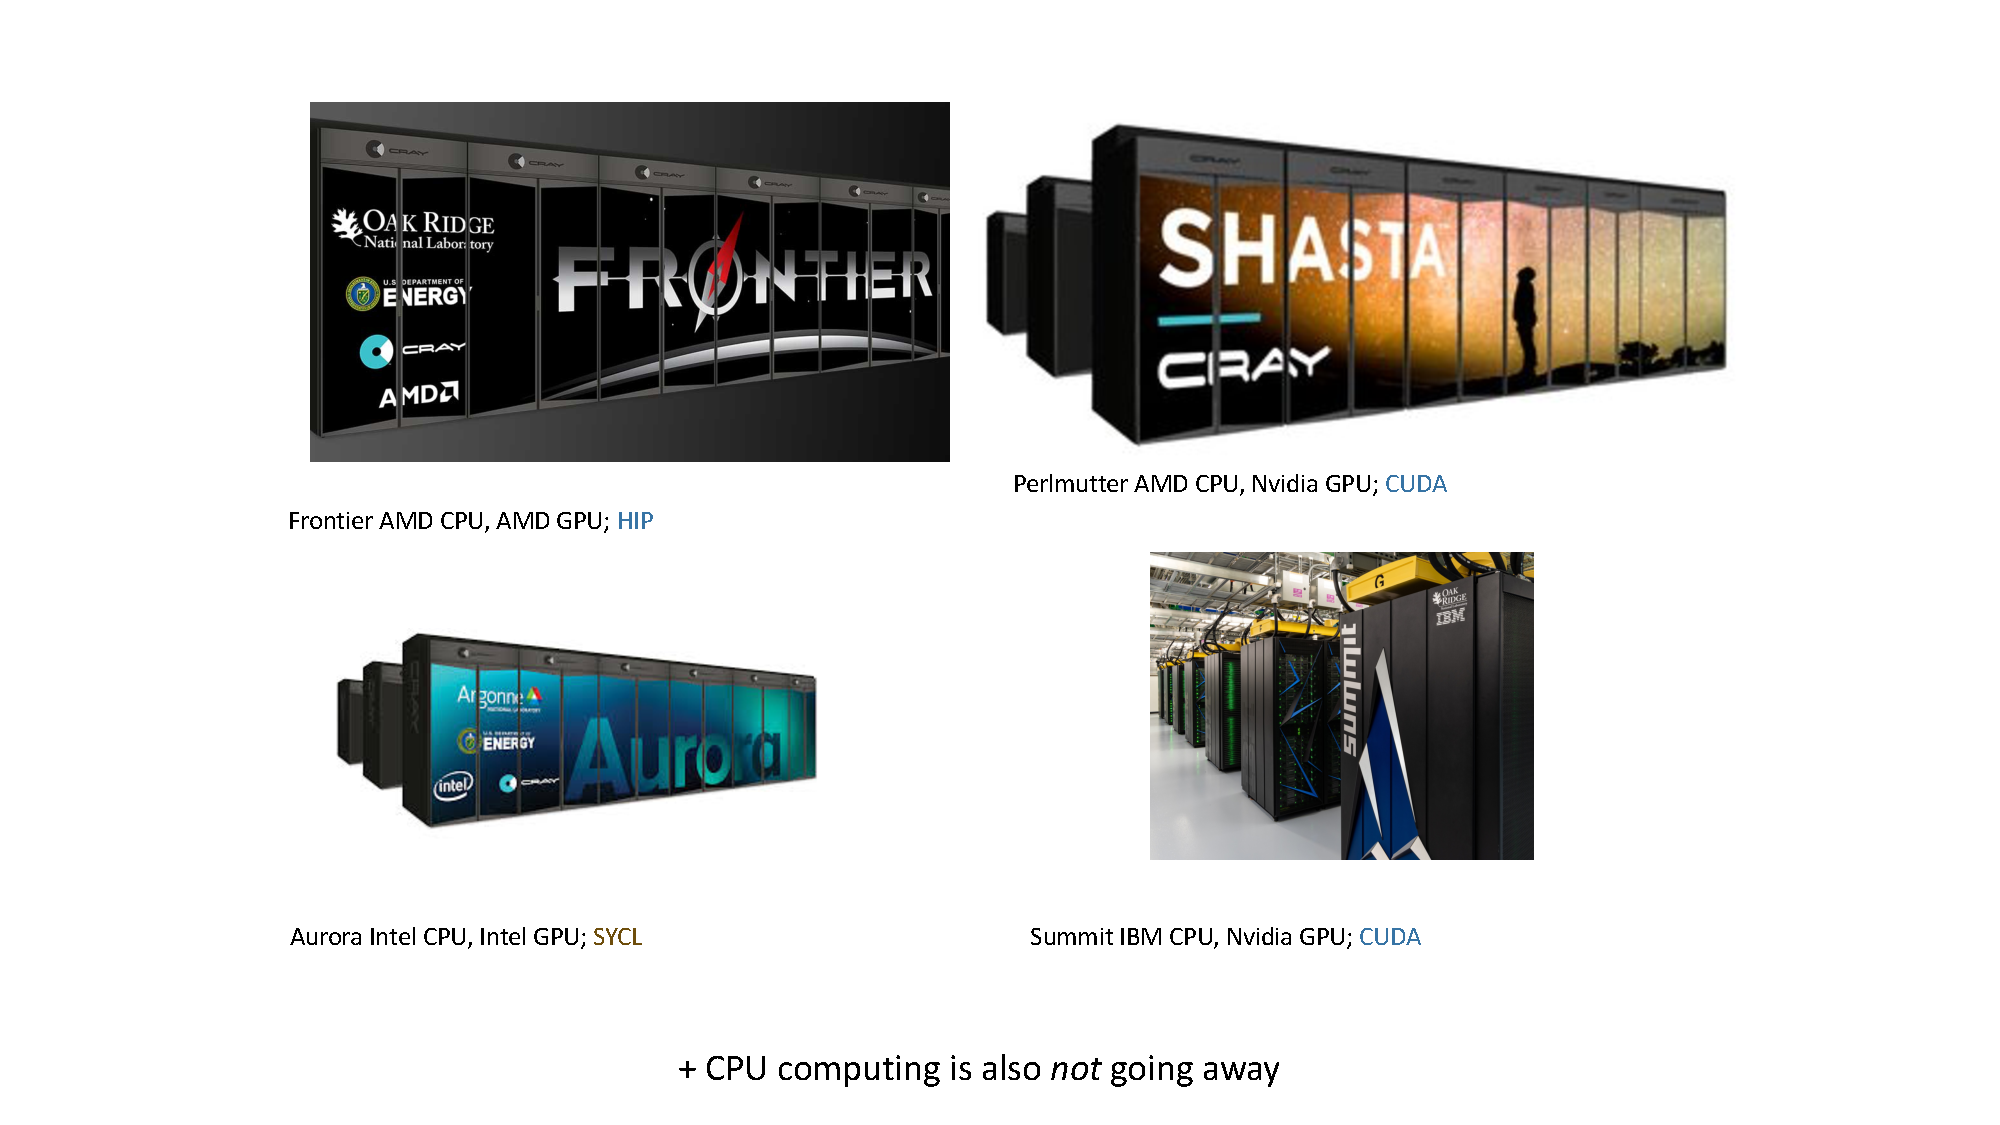
\includegraphics[width=0.8\textwidth]{Exascale.pdf}
\end{frame}

\begin{frame}[fragile]\small\frametitle{ Parallel computing and data parallel programming}

\includegraphics[width=0.8\textwidth]{CMfortran.pdf}

\begin{itemize}
  \item \link{https://longnow.org/essays/richard-feynman-connection-machine/}
  \item \link{https://people.csail.mit.edu/bradley/cm5docs/CMFortranProgrammingGuide.pdf}
  \item Compare with QDP++
  \item HPF failed due to poor performance over MPI: {\color{red}systematic stencil operation assistance}
\begin{itemize}
  \item \emph{PGAS will probably fail for the same reasons!}
\end{itemize}
\item Never break a high level operation into a specific ordering and expect language to reorder \\
      Entropy in action! Preserve higher level information
\end{itemize}
\end{frame}

\begin{frame}[fragile]\small\frametitle{ }
\includegraphics[width=\textwidth]{DPexample.pdf}
\end{frame}

\begin{frame}[fragile]\small\frametitle{ Sparse matrices, stencils \& PDEs}

  \begin{columns}
    \begin{column}{0.7\textwidth}
  \begin{itemize}
  \item Encode differential operators as discrete finite difference derivatives
  \item Think of as sparse matrices - typically band diagonal
  $$ M(x,y) = \frac{\delta_{x+\mu,y}+\delta_{x-\mu,y}-2\delta_{x,y}}{a^2} $$
  \item In typicaly PDE usage, discretisation schemes can be encoded via coefficients and a \emph{stencil}
  \item {\color{red}The \emph{stencil} is a geometric shape encoding the set of points $y$ that contribute to the operator at point $x$}
  \item This is translationally invariant and characteristic of a discretisation scheme.
  \item Naive Laplacian and Wilson Fermions have a $2 N_d + 1 $ point stencil
  \item Improved staggered Fermions n discretisations have a $4 N_d + 1 $ point stencil
  \item Fourier transformation $\Rightarrow$ phase factor on each term in the stencil defines the lattice Feynman rules
  \item More non-local actions allow higher order improvement \\
    (classical/perturbative/NP)\\
    c.f. Hamber-Wu, Naik terms.
  \end{itemize}
    \end{column}
    \begin{column}{0.3\textwidth}
      \includegraphics[width=\textwidth]{Stencil.pdf}

      2D Wilson stencil
      
      \includegraphics[width=\textwidth]{StencilNaik.pdf}

      Higher order derivative stencil

    \begin{eqnarray*}
      \begin{array}{c} c_1 (e^{ip_\mu} - e^{-ip_\mu}) \\ + c_2 (e^{i2 p_\mu} - e^{-i2 p_\mu})\end{array} \\
      \to  i p_\mu + O(p_\mu^5)
      \end{eqnarray*}
    \end{column}
  \end{columns}
\end{frame}

\begin{frame}[fragile]\small\frametitle{ Grids primitives (see documentation)}

  \begin{itemize}
  \item Common QCD discretisations suggest we can construct most operations with
    \begin{itemize}
  \item N-dimensional grids
  \item Shifting along coordinate axes
  \item Gauge covariant of shifting fields
  \item Cartesian stencil operators along axes only
  \item Generic stencil operators within some taxi-cab distance
  \item Site local arithmetic: matrix/vector/scalar addition, subtraction, multiplication, math library functions
  \item Reductions: Inner-product, norm2, volume sum, slice summing (N-1 dim)
  \item N-dim FFT
  \item BlockProjection/Promotion between coarse and fine grids
  \end{itemize}
  \end{itemize}

\end{frame}


\begin{frame}[fragile]\small\frametitle{ Example: Free and covariant Laplacian}
  \link{https://www.github.com/paboyle/Grid/examples/Example\_Laplacian.cc}
\begin{itemize}
\item  Base class \emph{defines an interface}.
\item  Specific derived classes inherit and implement this interface differently
\item  Algorithms deal with the base class and work with all derived operators
 \end{itemize}
{\tiny

\begin{verbatim}
/////////////////////////////////////////////////////////////////////////////////////////////
// Grid/algorithms/SparseMatrix.h: Interface defining general sparse matrix, such as a Fermion action
/////////////////////////////////////////////////////////////////////////////////////////////
template<class Field> class SparseMatrixBase {
public:
  virtual GridBase *Grid(void) =0;

  virtual void  M    (const Field &in, Field &out)=0;
  virtual void  Mdag (const Field &in, Field &out)=0;
  virtual void  MdagM(const Field &in, Field &out) {
    Field tmp (in.Grid());
    M(in,tmp);
    Mdag(tmp,out);
  }
};
  \end{verbatim}
}
\end{frame}

\begin{frame}[fragile]\small\frametitle{ Example: Free Laplacian (low performance)}

Introduce free field Cshift based Laplacian:

{\tiny
\begin{verbatim}
template<class Field> class FreeLaplacianCshift : public SparseMatrixBase<Field>
{
public:
  GridBase *grid;
  FreeLaplacianCshift(GridBase *_grid)
  {
    grid=_grid;
  };
  virtual GridBase *Grid(void) { return grid; };

  virtual void  M    (const Field &in, Field &out)
  {
    out = Zero();
    for(int mu=0;mu<Nd-1;mu++) {
      out = out + Cshift(in,mu,1) + Cshift(in,mu,-1) - 2.0 * in;
    }
  };
  virtual void  Mdag (const Field &in, Field &out) { M(in,out);}; // Laplacian is hermitian
};
  \end{verbatim}
}
\end{frame}


\begin{frame}[fragile]\small\frametitle{ Example: Covariant Laplacian (low performance)}


{\tiny
\begin{verbatim}
template<class Gimpl,class Field> class CovariantLaplacianCshift : public SparseMatrixBase<Field>
{
  INHERIT_GIMPL_TYPES(Gimpl);

  GridBase *grid;
  GaugeField U;
  
  CovariantLaplacianCshift(GaugeField &_U)    :    grid(_U.Grid()),    U(_U) {  };

  virtual void  M    (const Field &in, Field &out)
  {
    out=Zero();
    for(int mu=0;mu<Nd-1;mu++) {
      GaugeLinkField Umu = PeekIndex<LorentzIndex>(U, mu); // NB: Inefficent
      out = out + Gimpl::CovShiftForward(Umu,mu,in);    
      out = out + Gimpl::CovShiftBackward(Umu,mu,in);    
      out = out - 2.0*in;
    }
  };
  virtual void  Mdag (const Field &in, Field &out) { M(in,out);}; // Laplacian is hermitian
};
  \end{verbatim}
}
\begin{itemize}
\item The covariant shift is passed in through a policy template parameter class
\item Knowledge of boundary conditions is external: we've written Laplacian code that works for periodic \emph{and} charge conjugation boundary conditions
\item Wilson loops, Gauge actions, Fermion actions in Grid follow similar design ideas
\end{itemize}
\end{frame}

\begin{frame}[fragile]\small\frametitle{ Fourier test}

{\miniscule
\begin{verbatim}
  std:: cout << " Test A: compare in free Field to \"Feynman rule\" / Convolution theorem " <<std::endl;

  std::vector<int> dim_mask({1,1,1,0}); // 3d FFT

  FFT theFFT(&Grid);

  Field out(&Grid), F_out(&Grid), F_in(&Grid);

  // FFT the random input vector
  theFFT.FFT_dim_mask(F_in,in,dim_mask,FFT::forward);

  // Convolution theorem: multiply by Fourier representation of (discrete) Laplacian to apply diff op
  LatticeComplexD    lap(&Grid); lap = Zero();
  LatticeComplexD    kmu(&Grid); 

  for(int mu=0;mu<3;mu++) {

    RealD TwoPiL =  M_PI * 2.0/ latt_size[mu];

    LatticeCoordinate(kmu,mu);
    kmu = TwoPiL * kmu;

    // (e^ik_mu + e^-ik_mu - 2) = 2( cos kmu - 1) ~ 2 (1 - k_mu^2/2 -1 ) =k_mu^2 + O(k^4)
    lap = lap + 2.0*cos(kmu) - 2.0;
    
  }  
  F_out = lap * F_in;
  
  // Inverse FFT the result
  theFFT.FFT_dim_mask(out,F_out,dim_mask,FFT::backward);
  
  std::cout<<"Fourier xformed (in)             "<<norm2(F_in)<<std::endl;
  std::cout<<"Fourier xformed Laplacian x (in) "<<norm2(F_out)<<std::endl;
  
  std::cout<<"Momentum space Laplacian application  "<< norm2(out)<<std::endl;
  std::cout<<"Stencil Laplacian application         "<< norm2(out_CLcs)<<std::endl;
    
  diff = out_CLcs - out;
  std::cout<<"diff "<< norm2(diff)<<std::endl;
  \end{verbatim}
}
\end{frame}

\begin{frame}[fragile]\small\frametitle{Output}
  \begin{itemize}
  \item Compare to application in momentum space
    \begin{itemize}
      \item Textbook exercise; use to verify code on unit gauge + a random gauge transform of unit gauge
      \item Every Fermion action in Grid knows its own lattice Feynman rule and can \emph{self test} the free propagator
      \item In addition to regression to other code bases such as Chroma, Bagel or CPS
      \item Add gauge covariance and tests with all Gauge links being highly non-trivial are possible
    \end{itemize}
    \end{itemize}
  
{\tiny \begin{verbatim}
******************************************************************
 Test A: compare in free Field to "Feynman rule"  
******************************************************************
Fourier xformed (in)             1.25907e+07
Fourier xformed Laplacian x (in) 5.25498e+08
Momentum space Laplacian application  1.02636e+06
Stencil Laplacian application         1.02636e+06
diff 1.0201e-25
  \end{verbatim} 
}
\end{frame}

  \begin{frame}[fragile]\small\frametitle{ Gauge invariance test}
{\miniscule
  \begin{verbatim}
  std:: cout << "******************************************************************" <<std::endl;
  std:: cout << " Test B: gauge covariance  " <<std::endl;
  std:: cout << "******************************************************************" <<std::endl;

  LatticeGaugeField     U_GT(&Grid); // Gauge transformed field
  LatticeColourMatrix   g(&Grid);   // local Gauge xform matrix

  U_GT = U;
  // Make a random xform to teh gauge field
  SU<Nc>::RandomGaugeTransform(RNG,U_GT,g); // Unit gauge

  Field in_GT(&Grid); 
  Field out_GT(&Grid);

  Field out_CLcs_GT(&Grid);
  Field out_CLst_GT(&Grid);

  CovariantLaplacianCshift <PeriodicGimplR,Field> CLcs_GT(U_GT);
  CovariantLaplacianStencil<PeriodicGimplR,Field> CLst_GT(U_GT);

  in_GT  = g*in;
  out_GT = g*out_FLcs;

  // Check M^GT_xy in_GT = g(x) M_xy g^dag(y) g(y) in = g(x) out(x)
  CLcs_GT.M(in_GT,out_CLcs_GT);
  CLst_GT.M(in_GT,out_CLst_GT);

  diff = out_CLcs_GT - out_GT;
  std:: cout << " Difference between Gauge xformed result and covariant Cshift Laplacian in xformed gauge  = " <<norm2(diff)<<std::endl;

  diff = out_CLst_GT - out_GT;
  std:: cout << " Difference between Gauge xformed result and covariant Stencil Laplacian in xformed gauge  = " <<norm2(diff)<<std::endl;
  std:: cout << "--------------------------------------------------------" <<std::endl;
  \end{verbatim}
}
  \end{frame}

\begin{frame}[fragile]\small\frametitle{Output}
{\tiny \begin{verbatim}
******************************************************************
 Test B: gauge covariance  
******************************************************************
 Difference between Gauge xformed result and covariant Cshift Laplacian in xformed gauge  = 7.28706e-23
 Difference between Gauge xformed result and covariant Stencil Laplacian in xformed gauge  = 7.28985e-23
--------------------------------------------------------
  \end{verbatim}
}
\begin{itemize}
\item Covariance of operators is an reasonably strong check \\
      Many mistakes will break the gauge invariance
\item Hadronic correlation functions should be gauge invariant (ignore gauge fixed procedures)
\item Variations of this test are a common "test weapon of choice"\\
      A necessary {\bf but not sufficient} condition for correctness, loved by older LQCD scientists
\item { \color{red} The above two tests combined - correctness on a random gauge transform of free field prove the operator behaves
        as intended with non-unit random gauge links on every variable: {\bf a strong check} }
\end{itemize}
\end{frame}

  \begin{frame}[fragile]\small\frametitle{ Compare different implementations}

{\miniscule
  \begin{verbatim}

  FreeLaplacianCshift<Field>  FLcs(&Grid);
  FreeLaplacianStencil<Field> FLst(&Grid);

  LatticeGaugeField U(&Grid);
  SU<Nc>::ColdConfiguration(RNG,U);

  CovariantLaplacianCshift <PeriodicGimplR,Field> CLcs(U);
  CovariantLaplacianStencil<PeriodicGimplR,Field> CLst(U);

  std:: cout << " Test C: consistency of four different Laplacian implementations " <<std::endl;

  Field in(&Grid); gaussian(RNG,in);

  std:: cout << " Input test vector " <<norm2(in)<<std::endl;

  Field out_FLcs(&Grid);  Field out_FLst(&Grid);
  Field out_CLcs(&Grid);  Field out_CLst(&Grid);
  Field diff(&Grid);

  FLcs.M(in,out_FLcs);  
  FLst.M(in,out_FLst);
  CLcs.M(in,out_CLcs);
  CLst.M(in,out_CLst);
  std:: cout << "--------------------------------------------------------" <<std::endl;
  std:: cout << " Free cshift  output vector " <<norm2(out_FLcs)<<std::endl;
  std:: cout << " Free stencil output vector " <<norm2(out_FLst)<<std::endl;
  std:: cout << " Cov  cshift  output vector " <<norm2(out_CLcs)<<std::endl;
  std:: cout << " Cov  stencil output vector " <<norm2(out_CLst)<<std::endl;
  std:: cout << "--------------------------------------------------------" <<std::endl;

  diff = out_FLcs - out_FLst;
  std:: cout << " Difference between free Cshift Laplacian and free Stencil Laplacian      = " <<norm2(diff)<<std::endl;

  diff = out_FLcs - out_CLcs;
  std:: cout << " Difference between free Cshift Laplacian and covariant Cshift Laplacian  = " <<norm2(diff)<<std::endl;

  diff = out_FLcs - out_CLst;
  std:: cout << " Difference between free Cshift Laplacian and covariant Stencil Laplacian = " <<norm2(diff)<<std::endl;
  std:: cout << "--------------------------------------------------------" <<std::endl;

  \end{verbatim}
}
  \end{frame}

\begin{frame}[fragile]\small\frametitle{Output}
{\tiny \begin{verbatim}
******************************************************************
 Test C: consistency of four different Laplacian implementations 
******************************************************************
 Input test vector 24591.2
--------------------------------------------------------
 Free cshift  output vector 1.02636e+06
 Free stencil output vector 1.02636e+06
 Cov  cshift  output vector 1.02636e+06
 Cov  stencil output vector 1.02636e+06
--------------------------------------------------------
 Difference between free Cshift Laplacian and free Stencil Laplacian      = 2.2926e-26
 Difference between free Cshift Laplacian and covariant Cshift Laplacian  = 0
 Difference between free Cshift Laplacian and covariant Stencil Laplacian = 2.2926e-26
--------------------------------------------------------
\end{verbatim}
}
  \begin{itemize}
  \item Stencil vs. Cshift based cross checked.
  \item Free and covariant implementations on unit gauge 
  \item Can also compare different code bases (Chroma/CPS/Bagel/QUDA etc...)
  \begin{itemize}
  \item Weak to a common error (e.g. copy the same Dirac basis?), not scientifically independent
  \end{itemize}
  \item The Wilson and DWF type actions in Grid have been tested in the above fashion
  \item Caution: the Clover field strengh is identically zero in a transform of free field
  \end{itemize}

  \end{frame}

\begin{frame}[fragile]\small\frametitle{Exercise}
\begin{itemize}
\item Obtain and compile Grid;
\item Read and run the example
\begin{verbatim}
git clone https://www.github.com/paboyle/Grid
cd Grid
./bootstrap.sh
mkdir build
cd build
../configure --enable-simd=GEN --enable-debug
make -j 8
cd examples
./Example_Laplacian
\end{verbatim}
\end{itemize}
\end{frame}


\end{document}



